\mc
\section{機械の整備}
今回作成したロボットはパーツの点数が多く,持ち運ぶ際に分解した後の組み立てに時間がかかる.そこでロボットを駆動部である2つのDモジュールと中心部のCモジュールに分解させることで,最小限の分解で持ち運びを容易に行えるように設計した.これにより組み立ての時間を短縮することが狙いである
\subsection{必要な工具}
ロボットを分解,組み立てする際に必要な工具を以下に示す.基本的に全サイズを用意しておく.
\begin{enumerate}
 \item 六角レンチ
 \item レンチ
\end{enumerate}

\section{分解方法}
以下に分解手順を示す.本分解方法はつくばチャレンジ2016に参加した際に用いた方法と同様のものである.また,前提として上面のアクリル板に設置されたセンサ類のコードはすべて外してあり,別途に確保してある状態とする.
\begin{figure}[htp]
 \begin{center}
  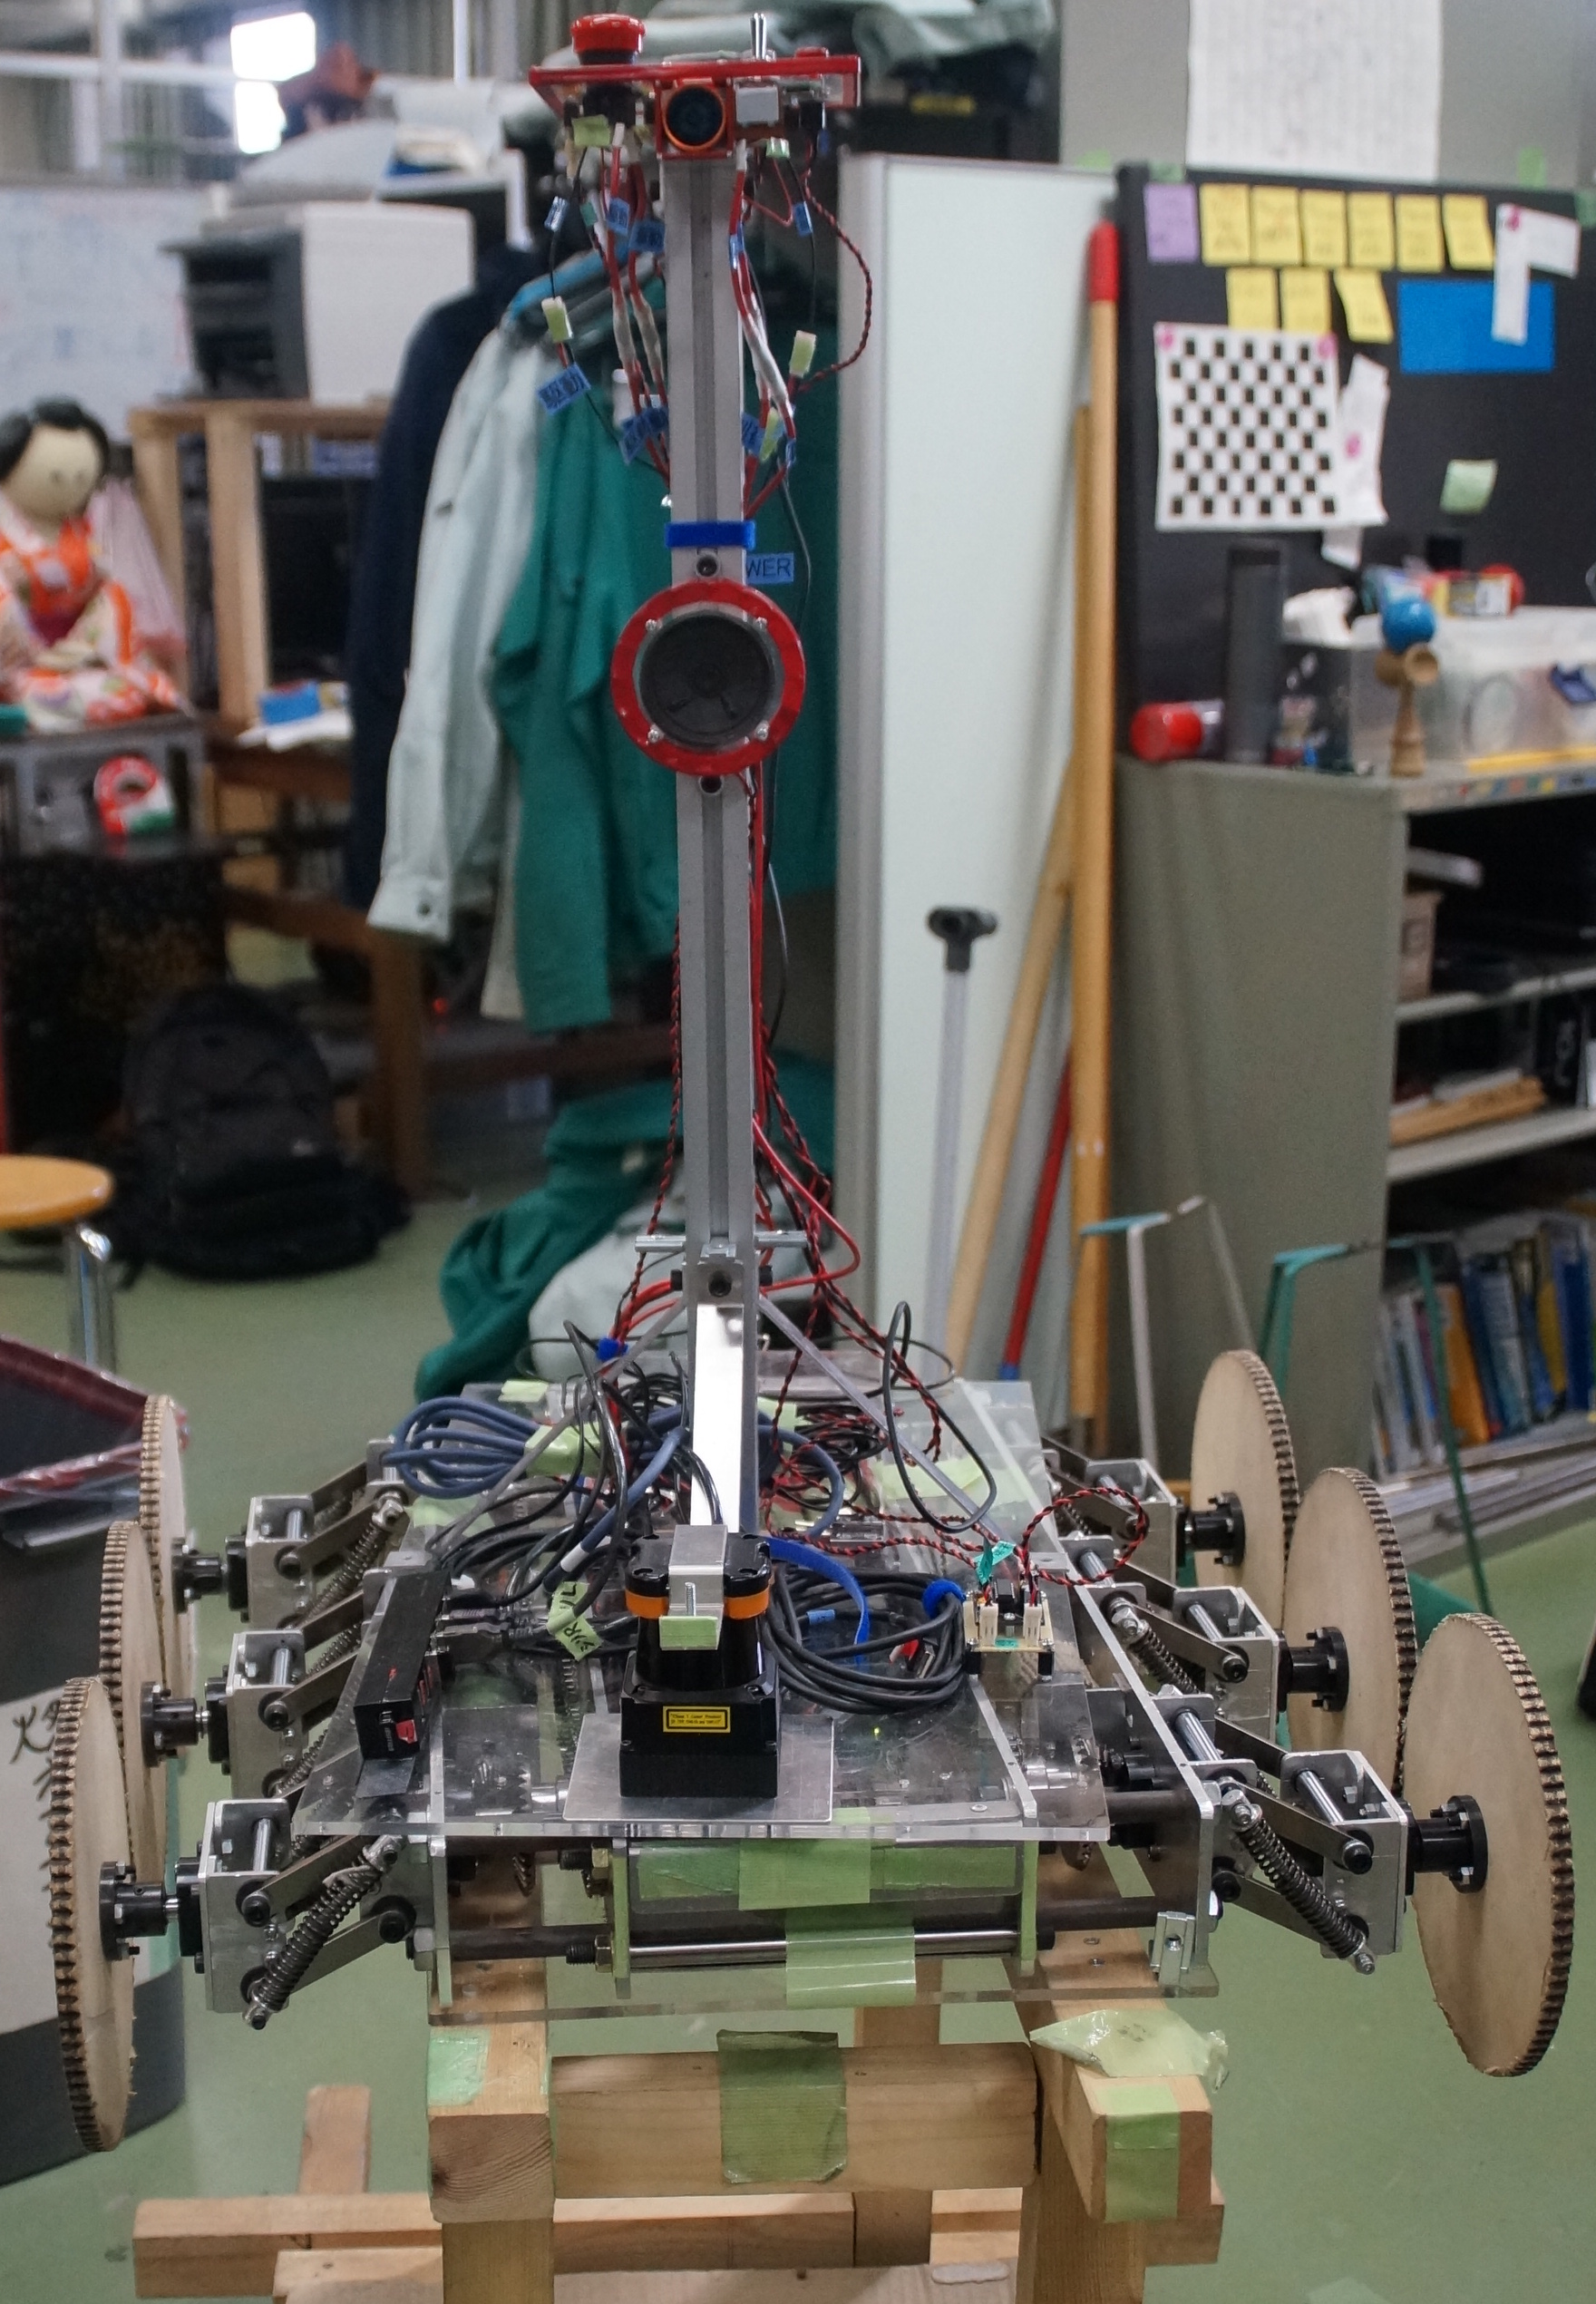
\includegraphics[width=80mm]{img/hard/f13.jpg}
  \caption{ロボット図}
  \label{fig:robot}%ここに文章中で使用する名前を指定する
 \end{center}
\end{figure}

\subsection{ポールとアクリル板の取り外し}
ロボット上面のアクリル板はM3の六角穴付ボルトを使用している.ポールはM6の六角穴付ボルトとM3のボルトを使用している.

\begin{enumerate}
 \item アクリル板に取り付けてあるM3ボルトを全て取り外す.
 \item ポールのコード類が外されていることを確認し,アクリル板とポールを取り外す.(このときポールはアクリル板に固定されている状態である)
 \item ロボットをひっくり返し,腹面のアクリル板も同様に取り外す.
\end{enumerate}
なおポールそのものを持っての運搬,それに当たる行為は禁止である.アクリル板を落下し破損させる恐れがある.

\begin{figure}[htp]
 \begin{center}
  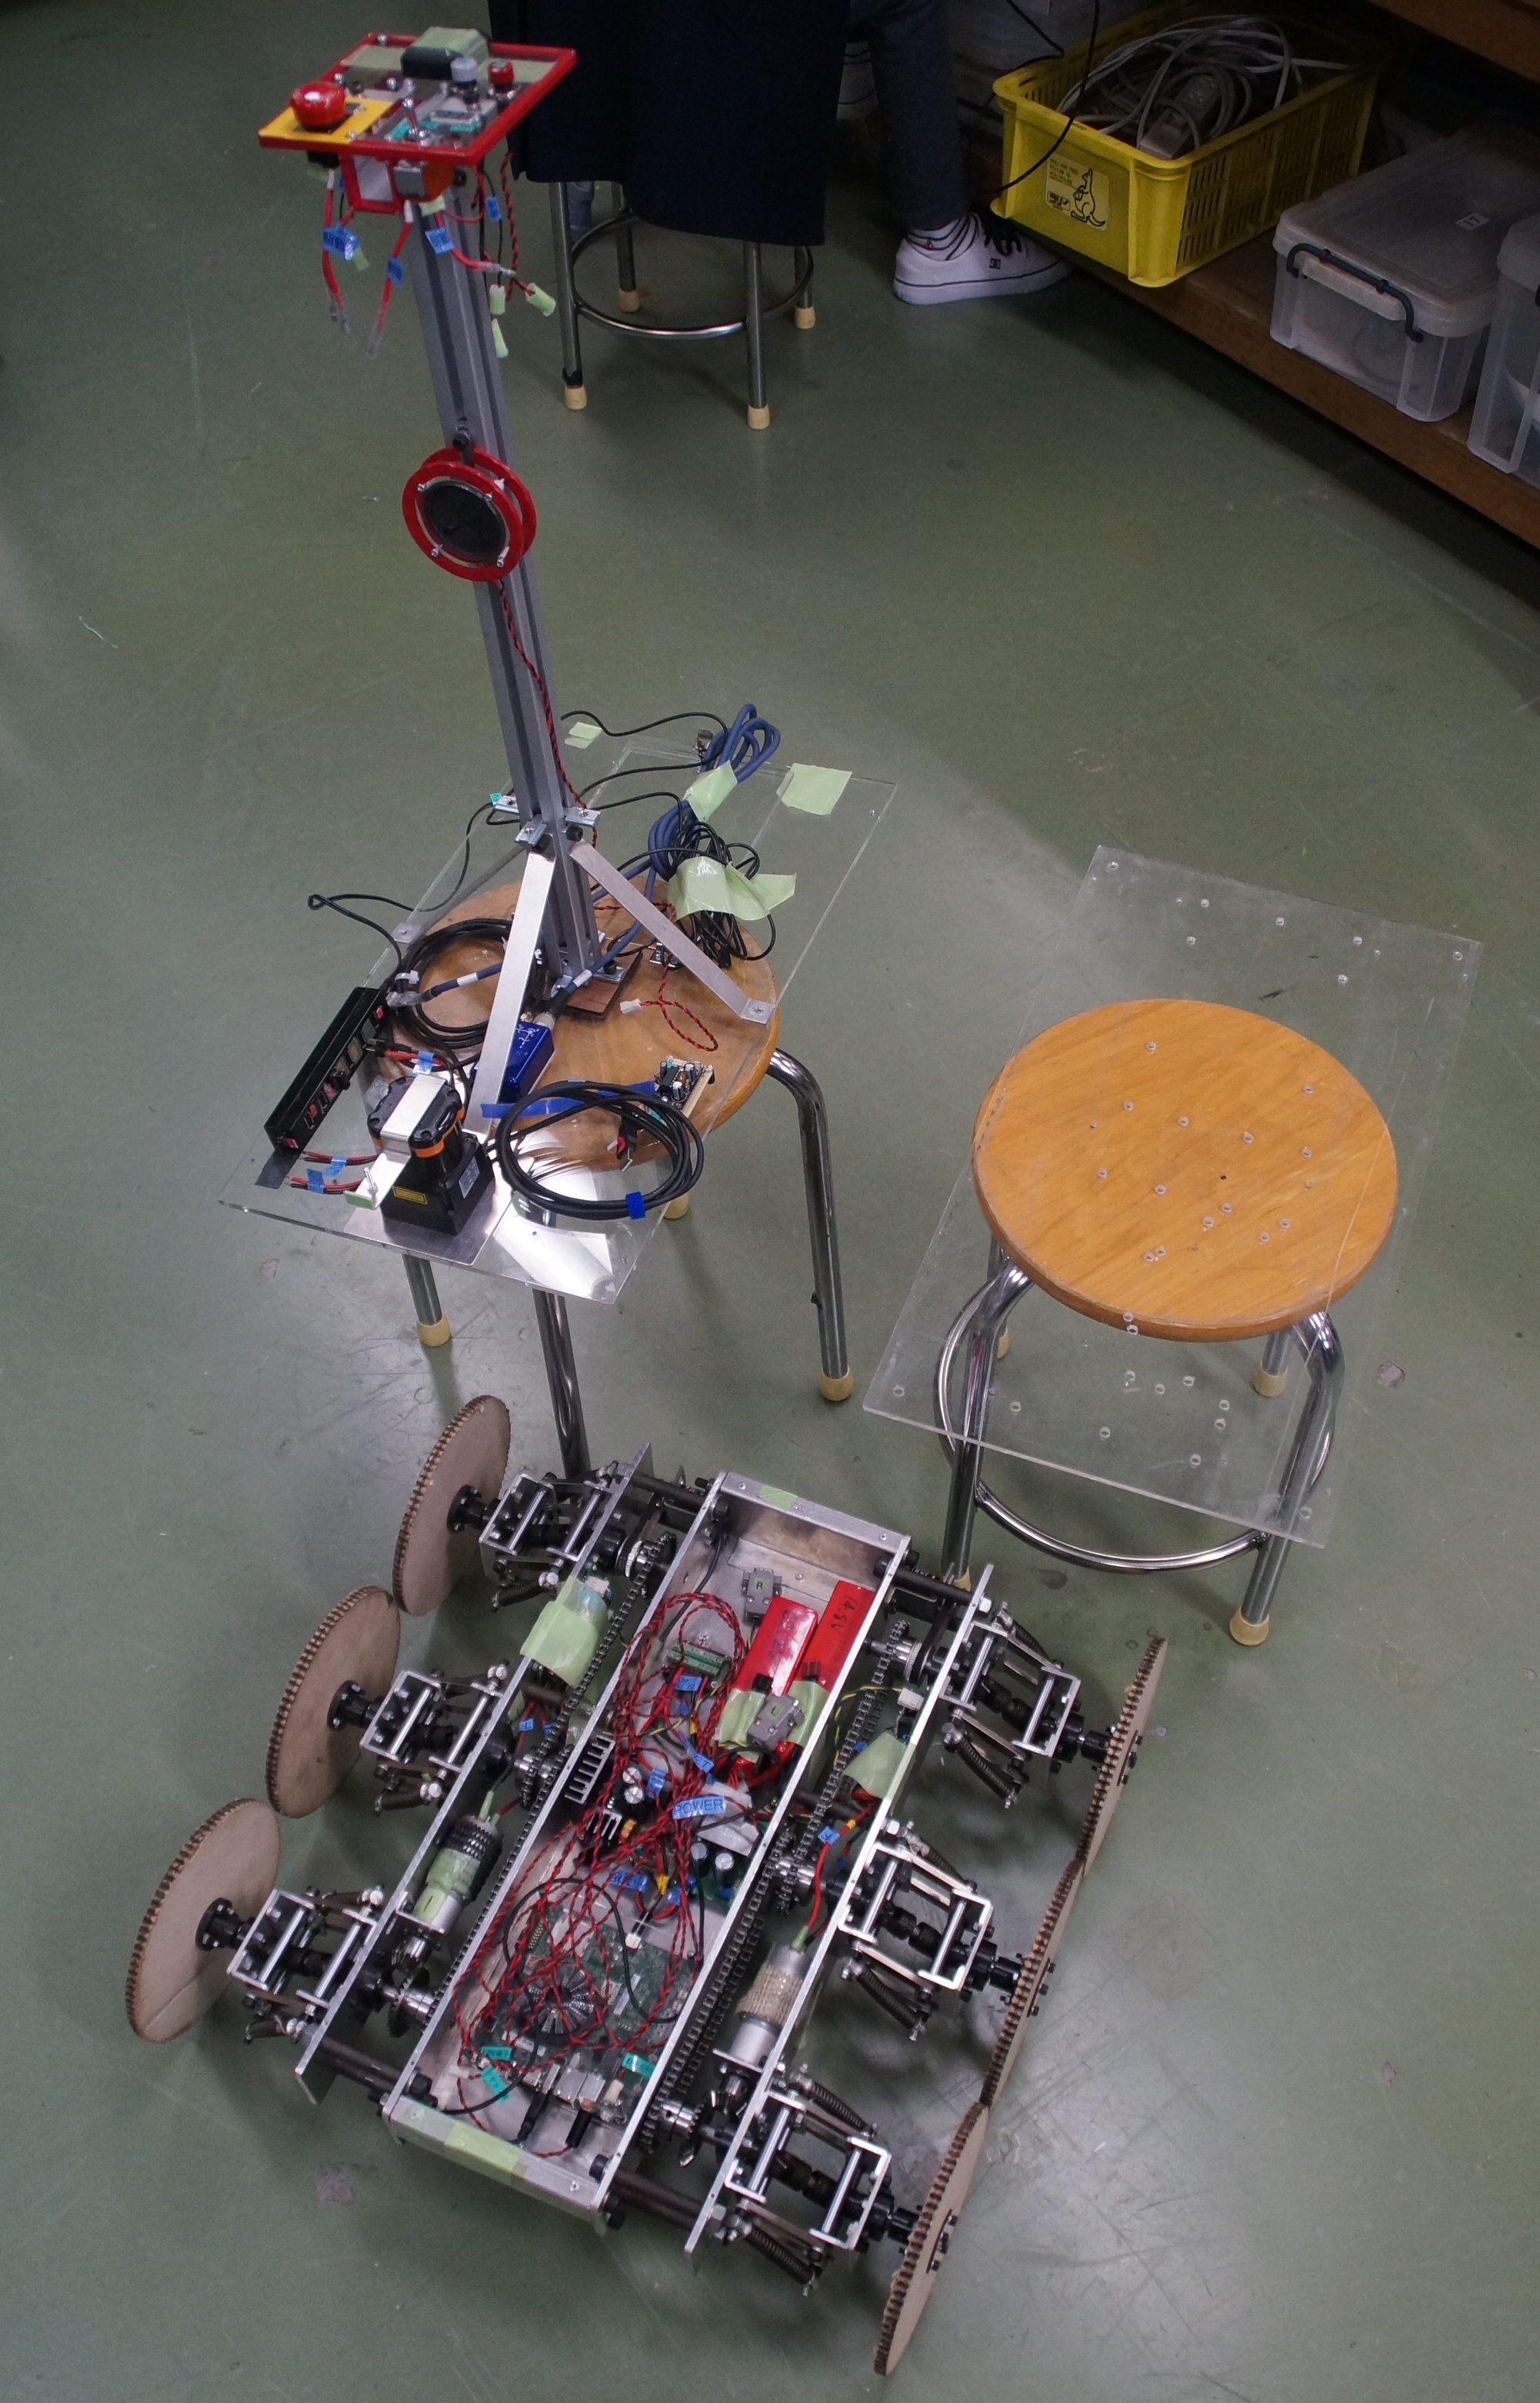
\includegraphics[width=80mm]{img/hard/f11.jpg}
  \caption{分解図}
  \label{fig:bunkai1}%ここに文章中で使用する名前を指定する
 \end{center}
\end{figure}



\subsection{DモジュールとCモジュールの分解}
この分解はDモジュールに接続されているコード類を引きちぎらないように注意を払って分解する.
ロボットの中心に保持されている部分がCモジュールである.CモジュールはM8の六角穴付ボルト4本で2つのDモジュールと接続されている
\begin{enumerate}
 \item M8ボルトを全て取り外し,Dモジュールを横に少し引き出す
 \item Dモジュールに接続されたシリアルケーブル(緑黄),電源ケーブル(赤黒),エンコーダケーブル(黒)を取り外す
 \item Dモジュールを完全に引き出し,Cモジュールを取り出す
\end{enumerate}
使用されているM8ボルトはDモジュールと一体化しているが問題はない,またカラーを無くさないようにする.くれぐれもコード類を引きちぎらないように注意する

\begin{figure}[htp]
 \begin{center}
  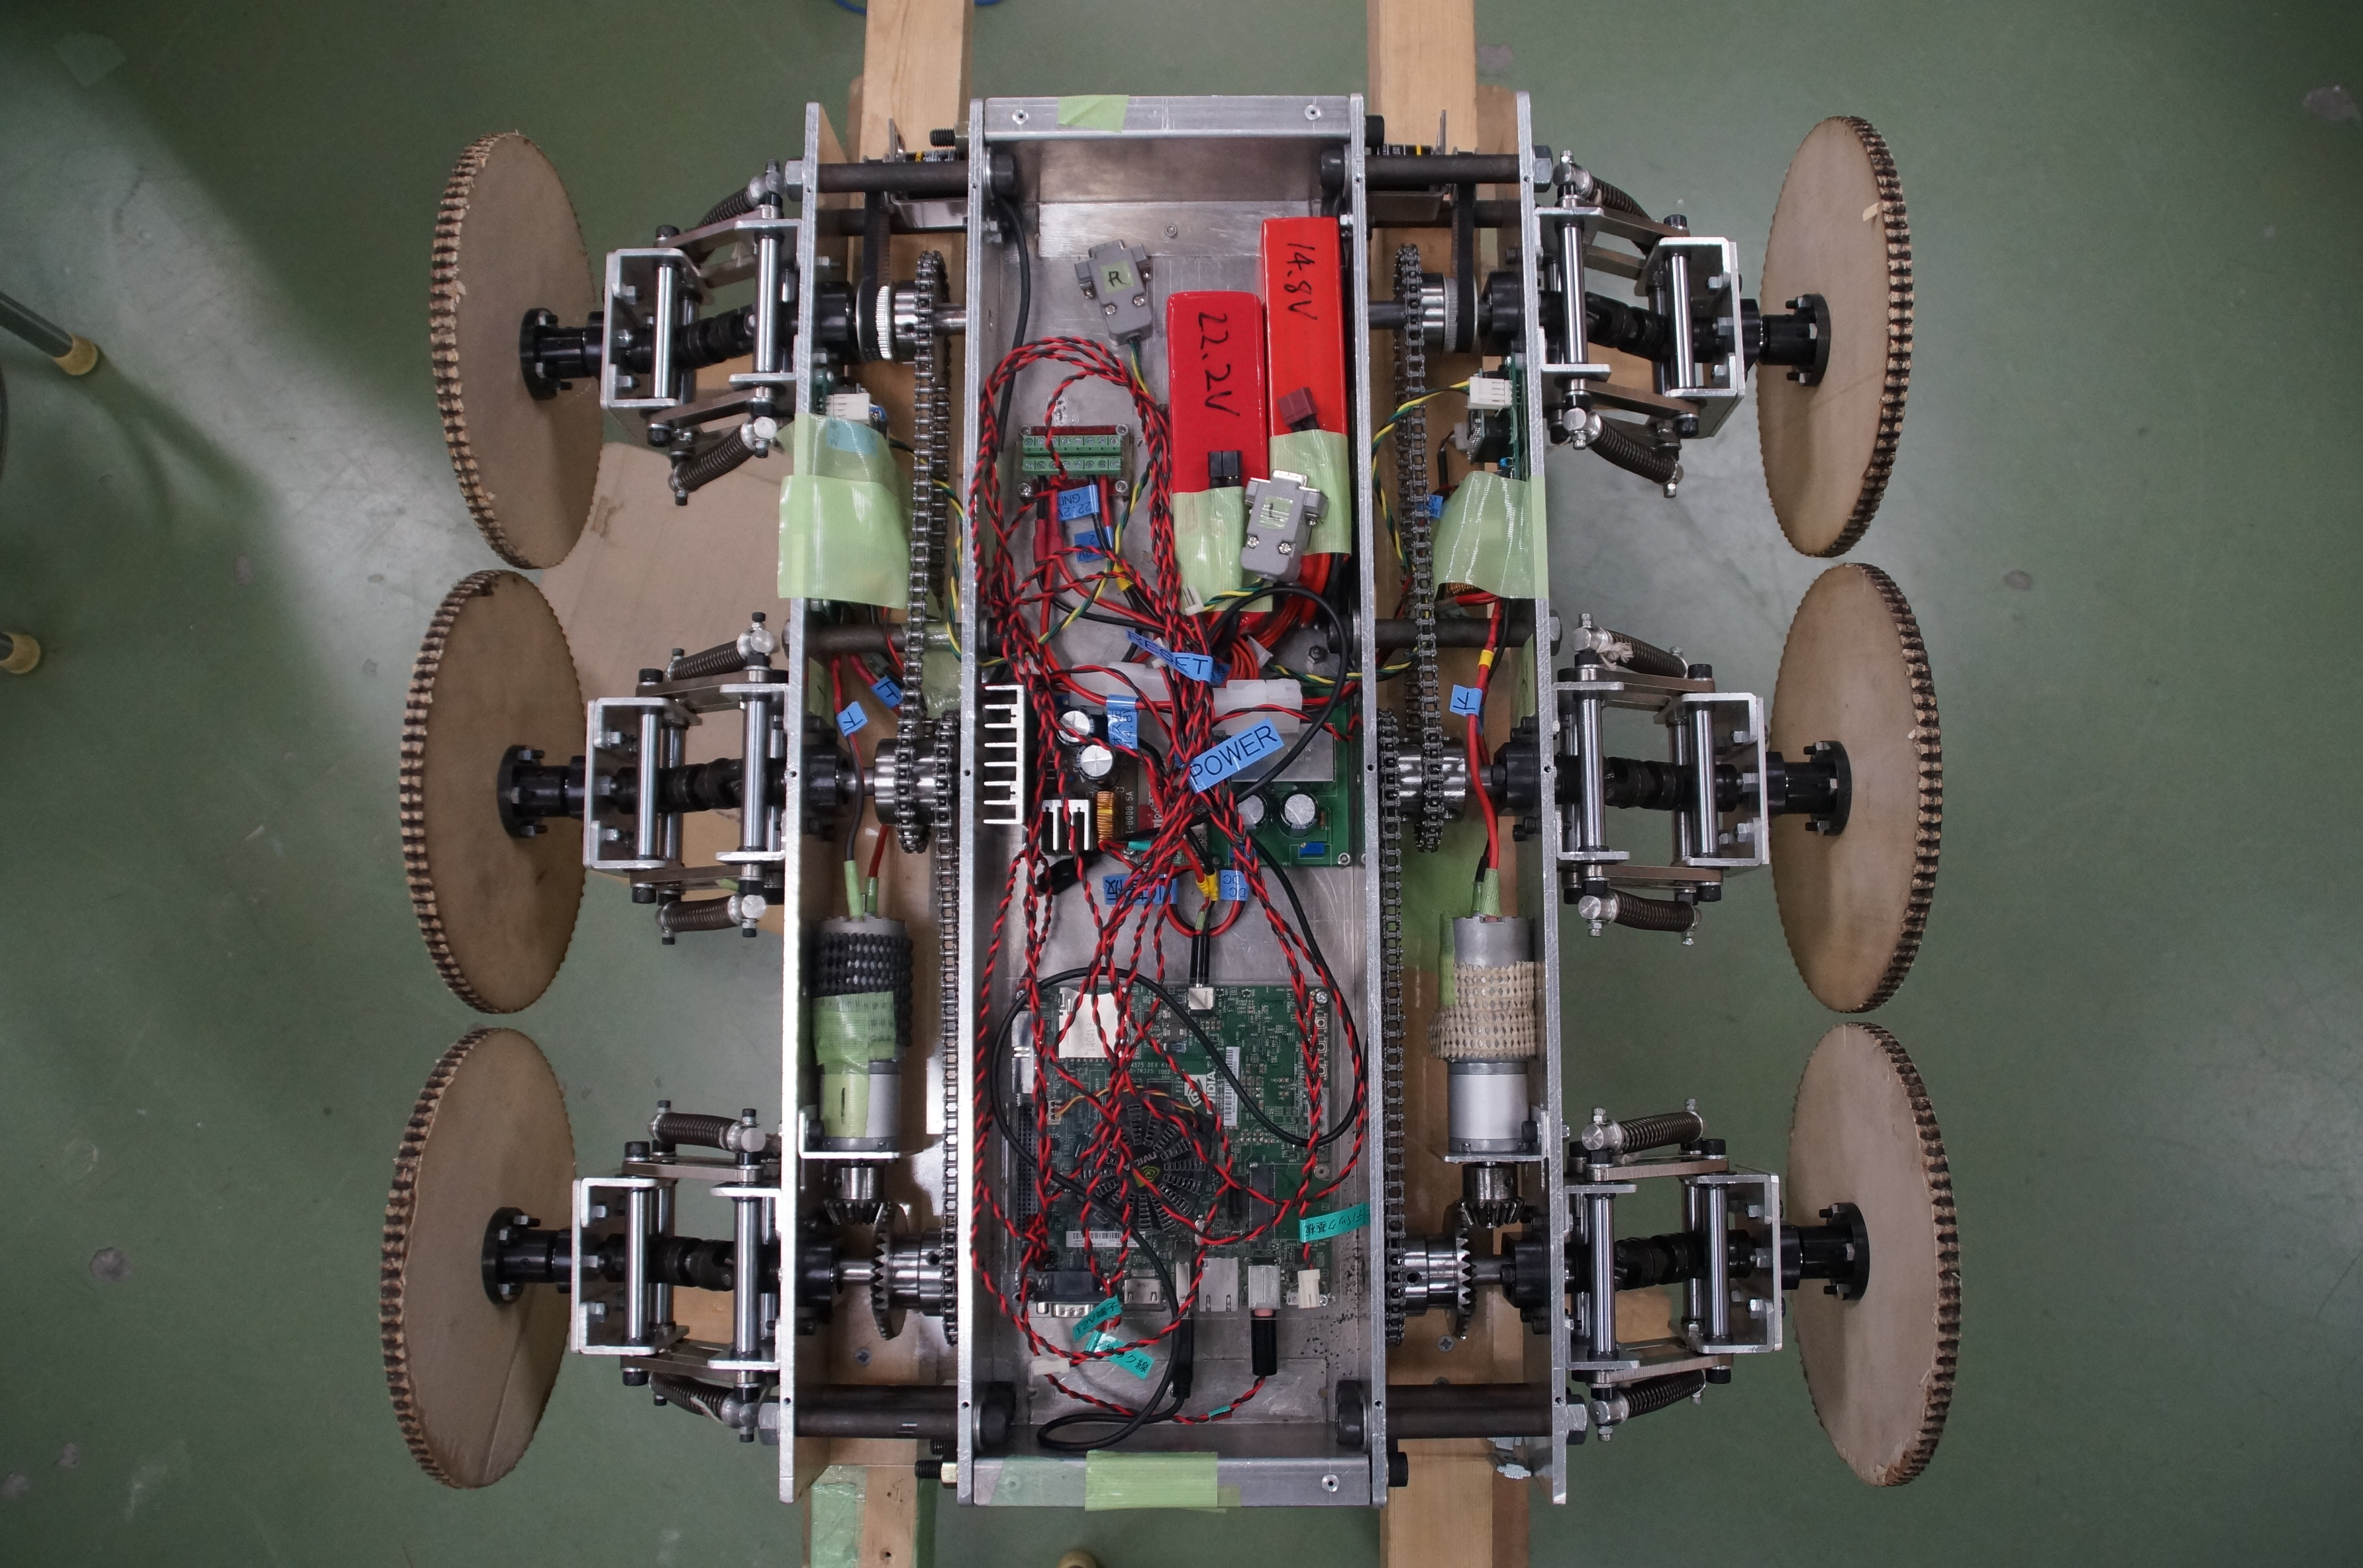
\includegraphics[width=80mm]{img/hard/f12.jpg}
  \caption{分解図}
  \label{fig:robot}%ここに文章中で使用する名前を指定する
 \end{center}
\end{figure}


\begin{figure}[htp]
 \begin{center}
  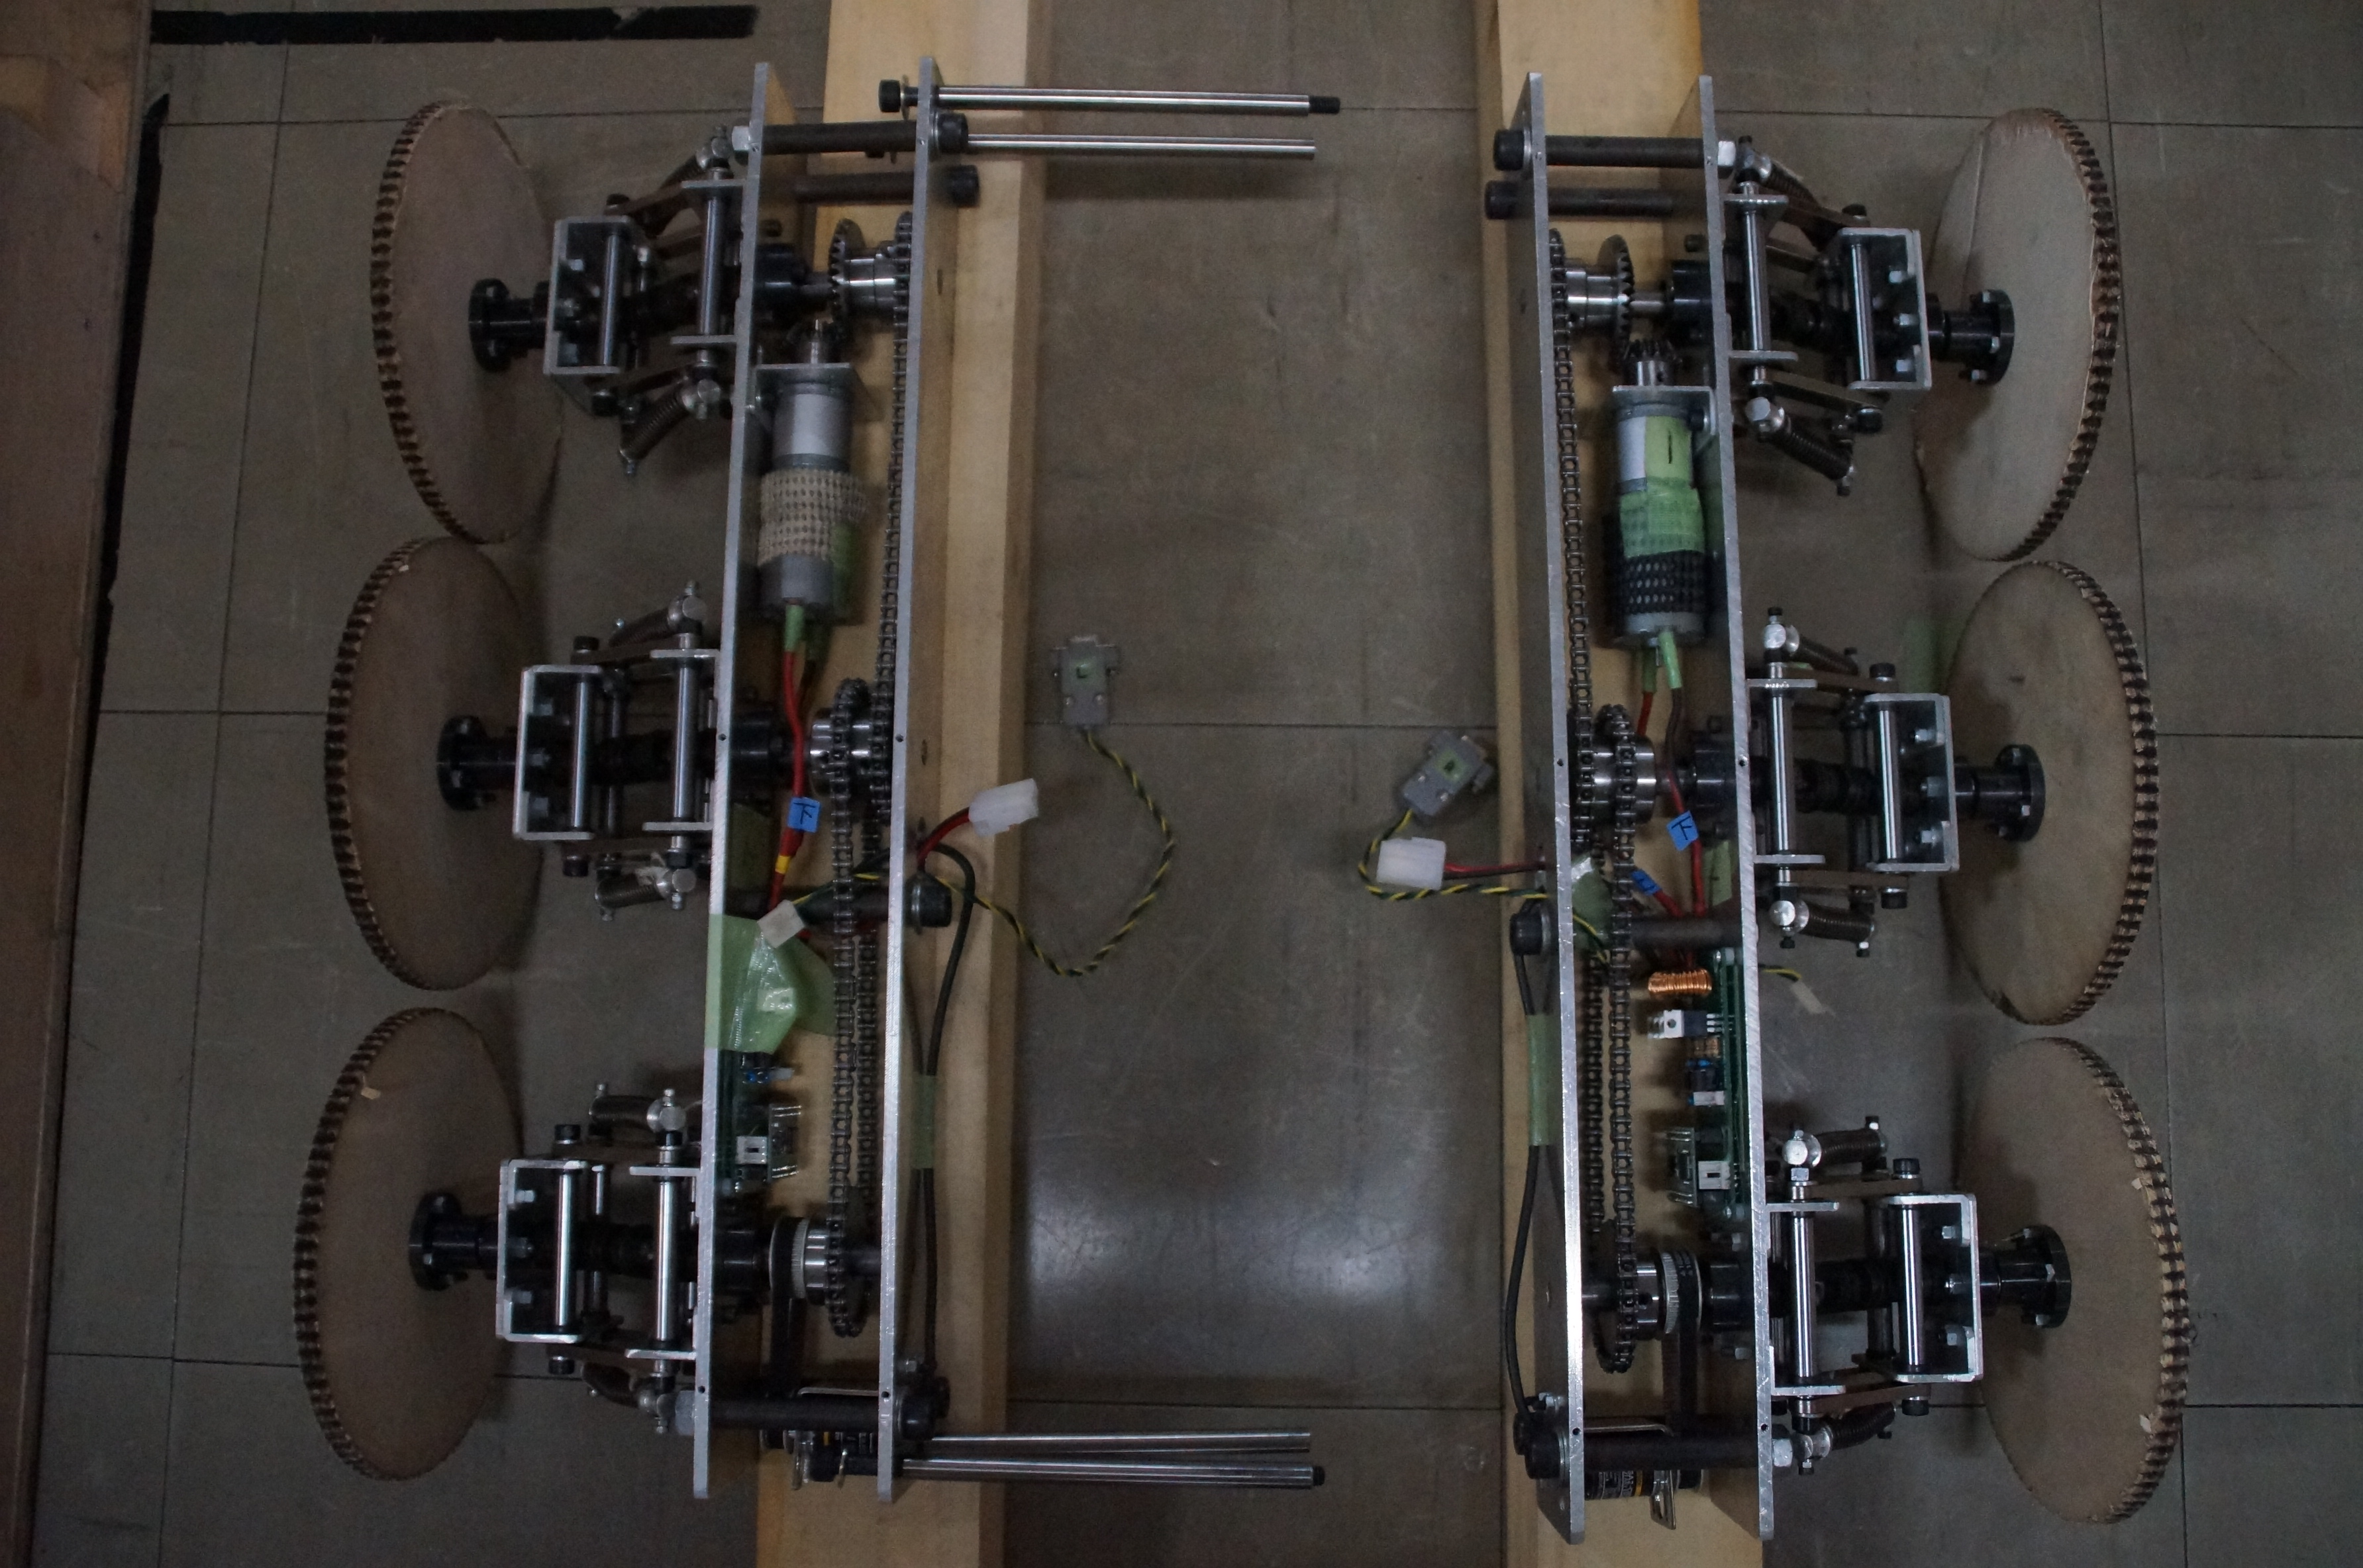
\includegraphics[width=80mm]{img/hard/f10.jpg}
  \caption{分解図}
  \label{fig:robot}%ここに文章中で使用する名前を指定する
 \end{center}
\end{figure}

\begin{figure}[htp]
 \begin{center}
  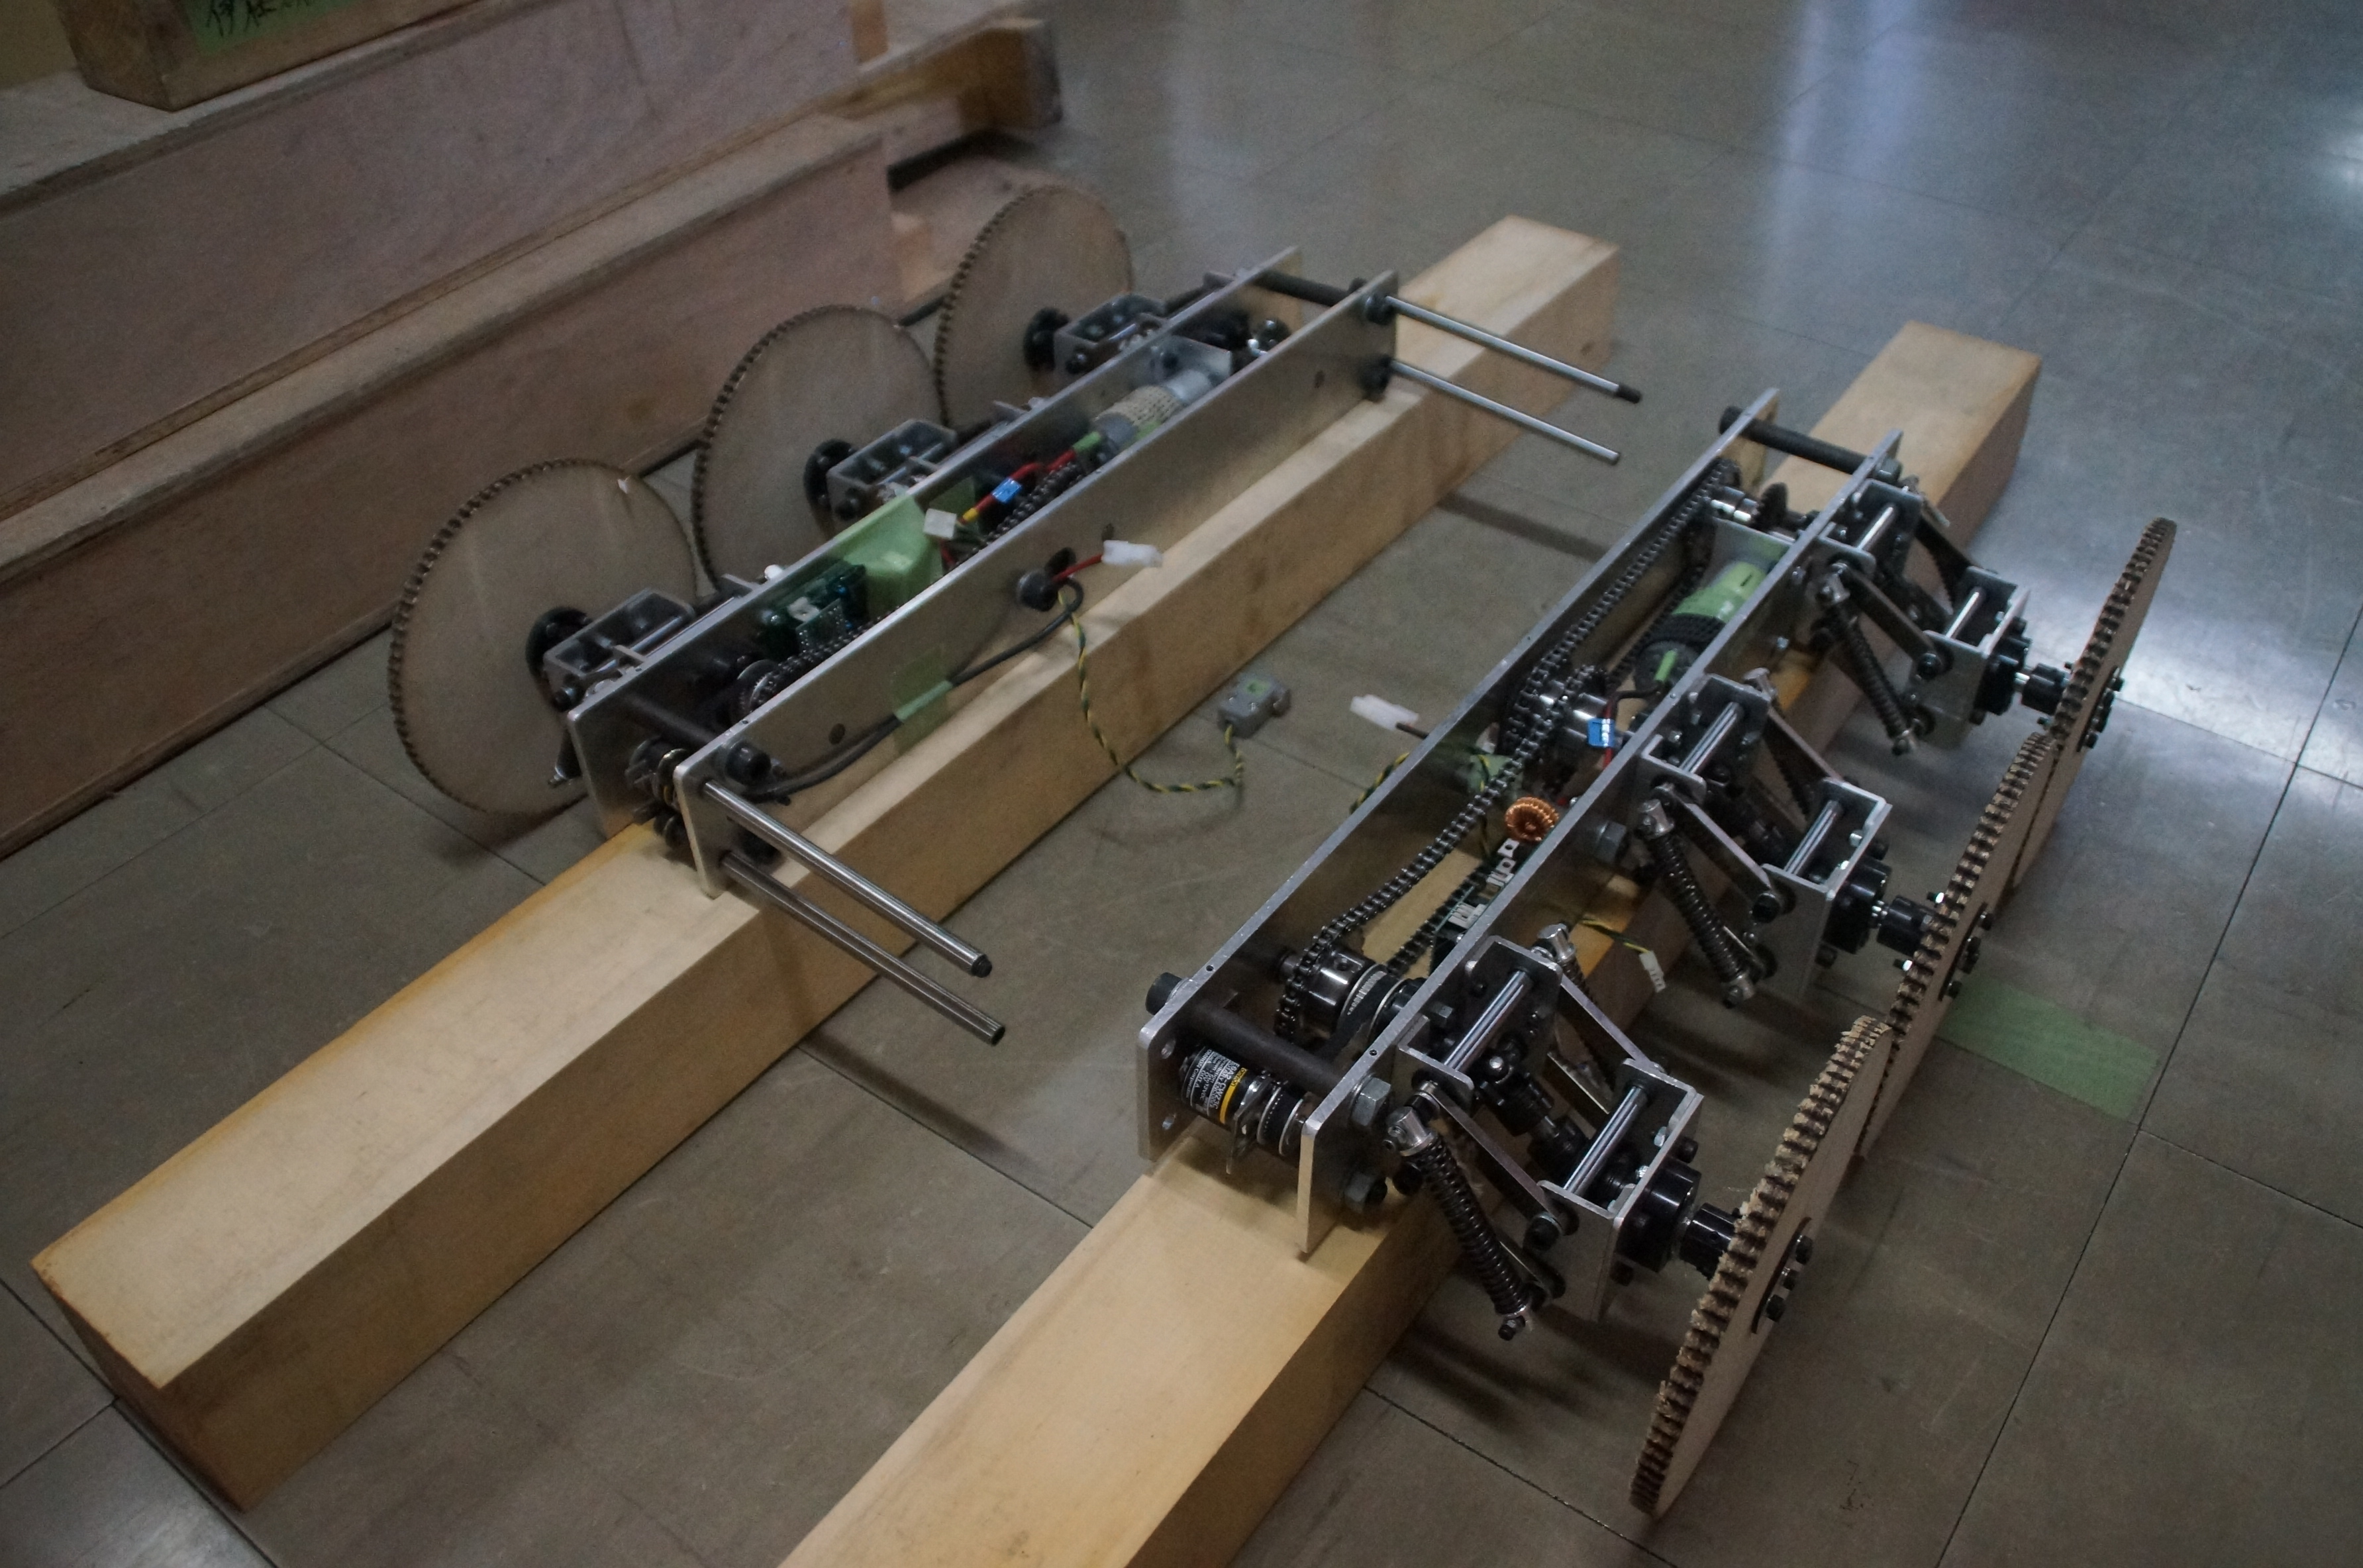
\includegraphics[width=80mm]{img/hard/f9.jpg}
  \caption{分解図}
  \label{fig:robot}%ここに文章中で使用する名前を指定する
 \end{center}
\end{figure}


\begin{figure}[htp]
 \begin{center}
  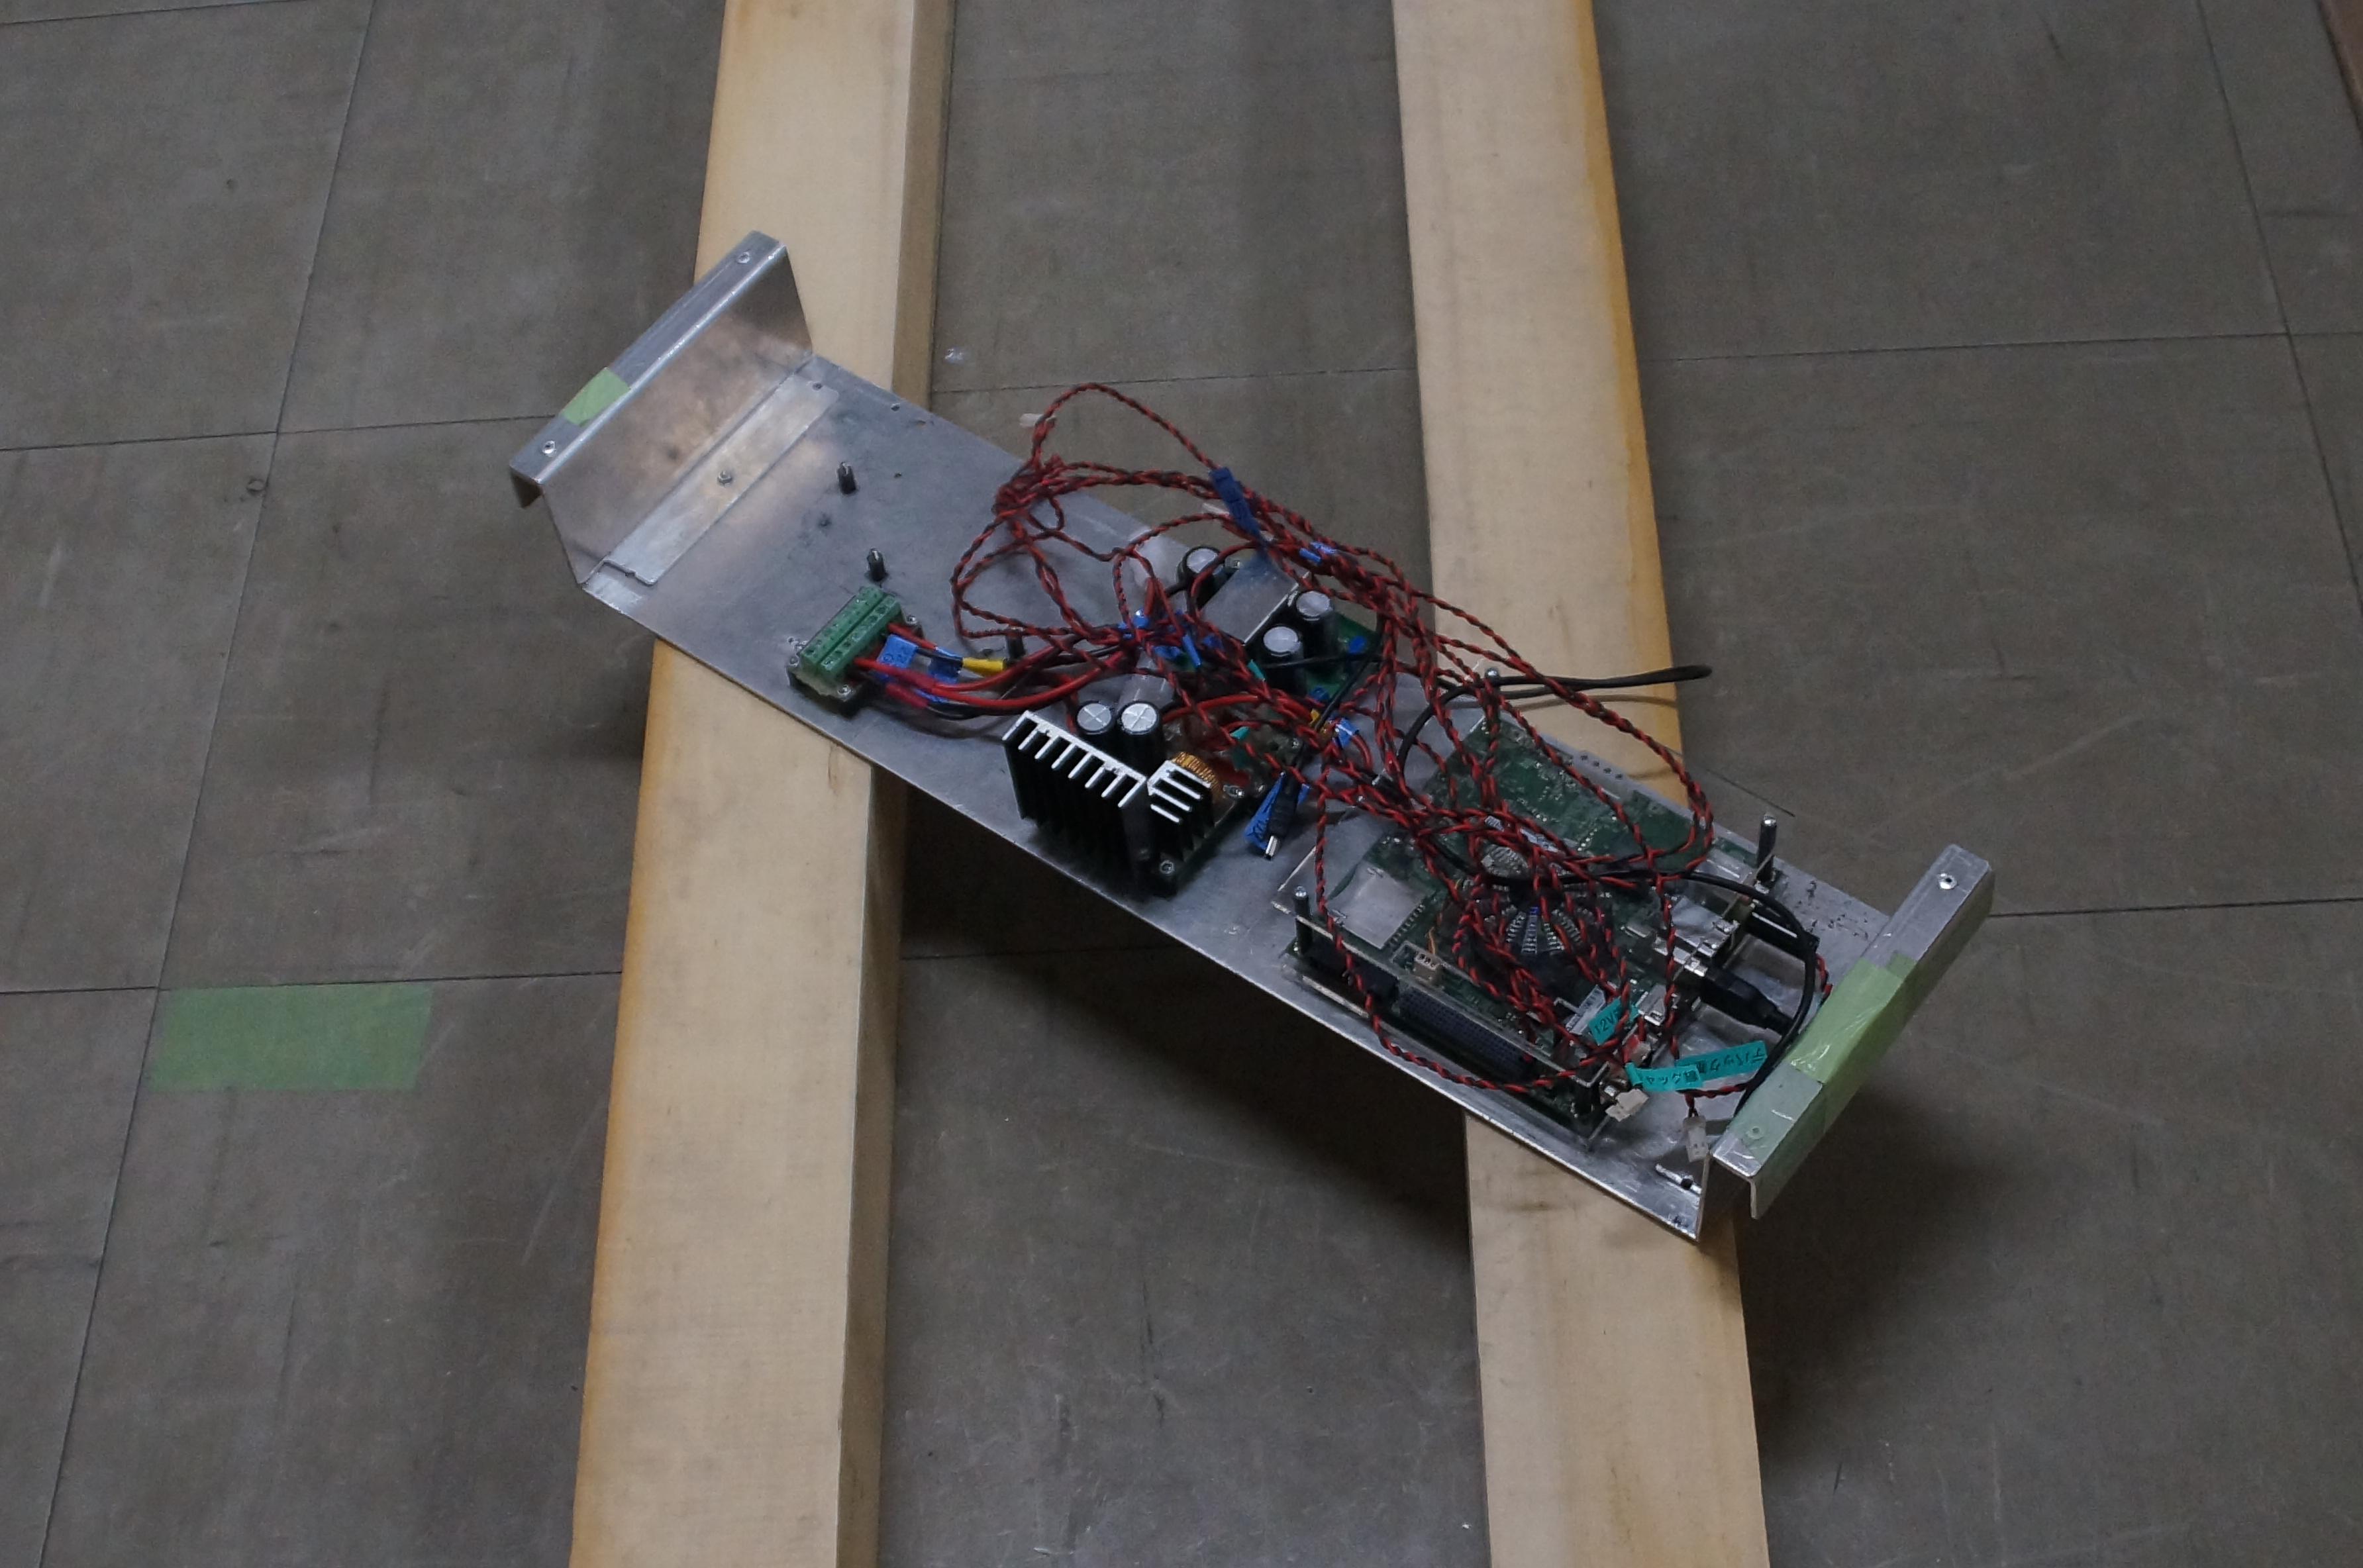
\includegraphics[width=80mm]{img/hard/f8.jpg}
  \caption{分解図}
  \label{fig:robot}%ここに文章中で使用する名前を指定する
 \end{center}
\end{figure}


\begin{figure}[htp]
 \begin{center}
  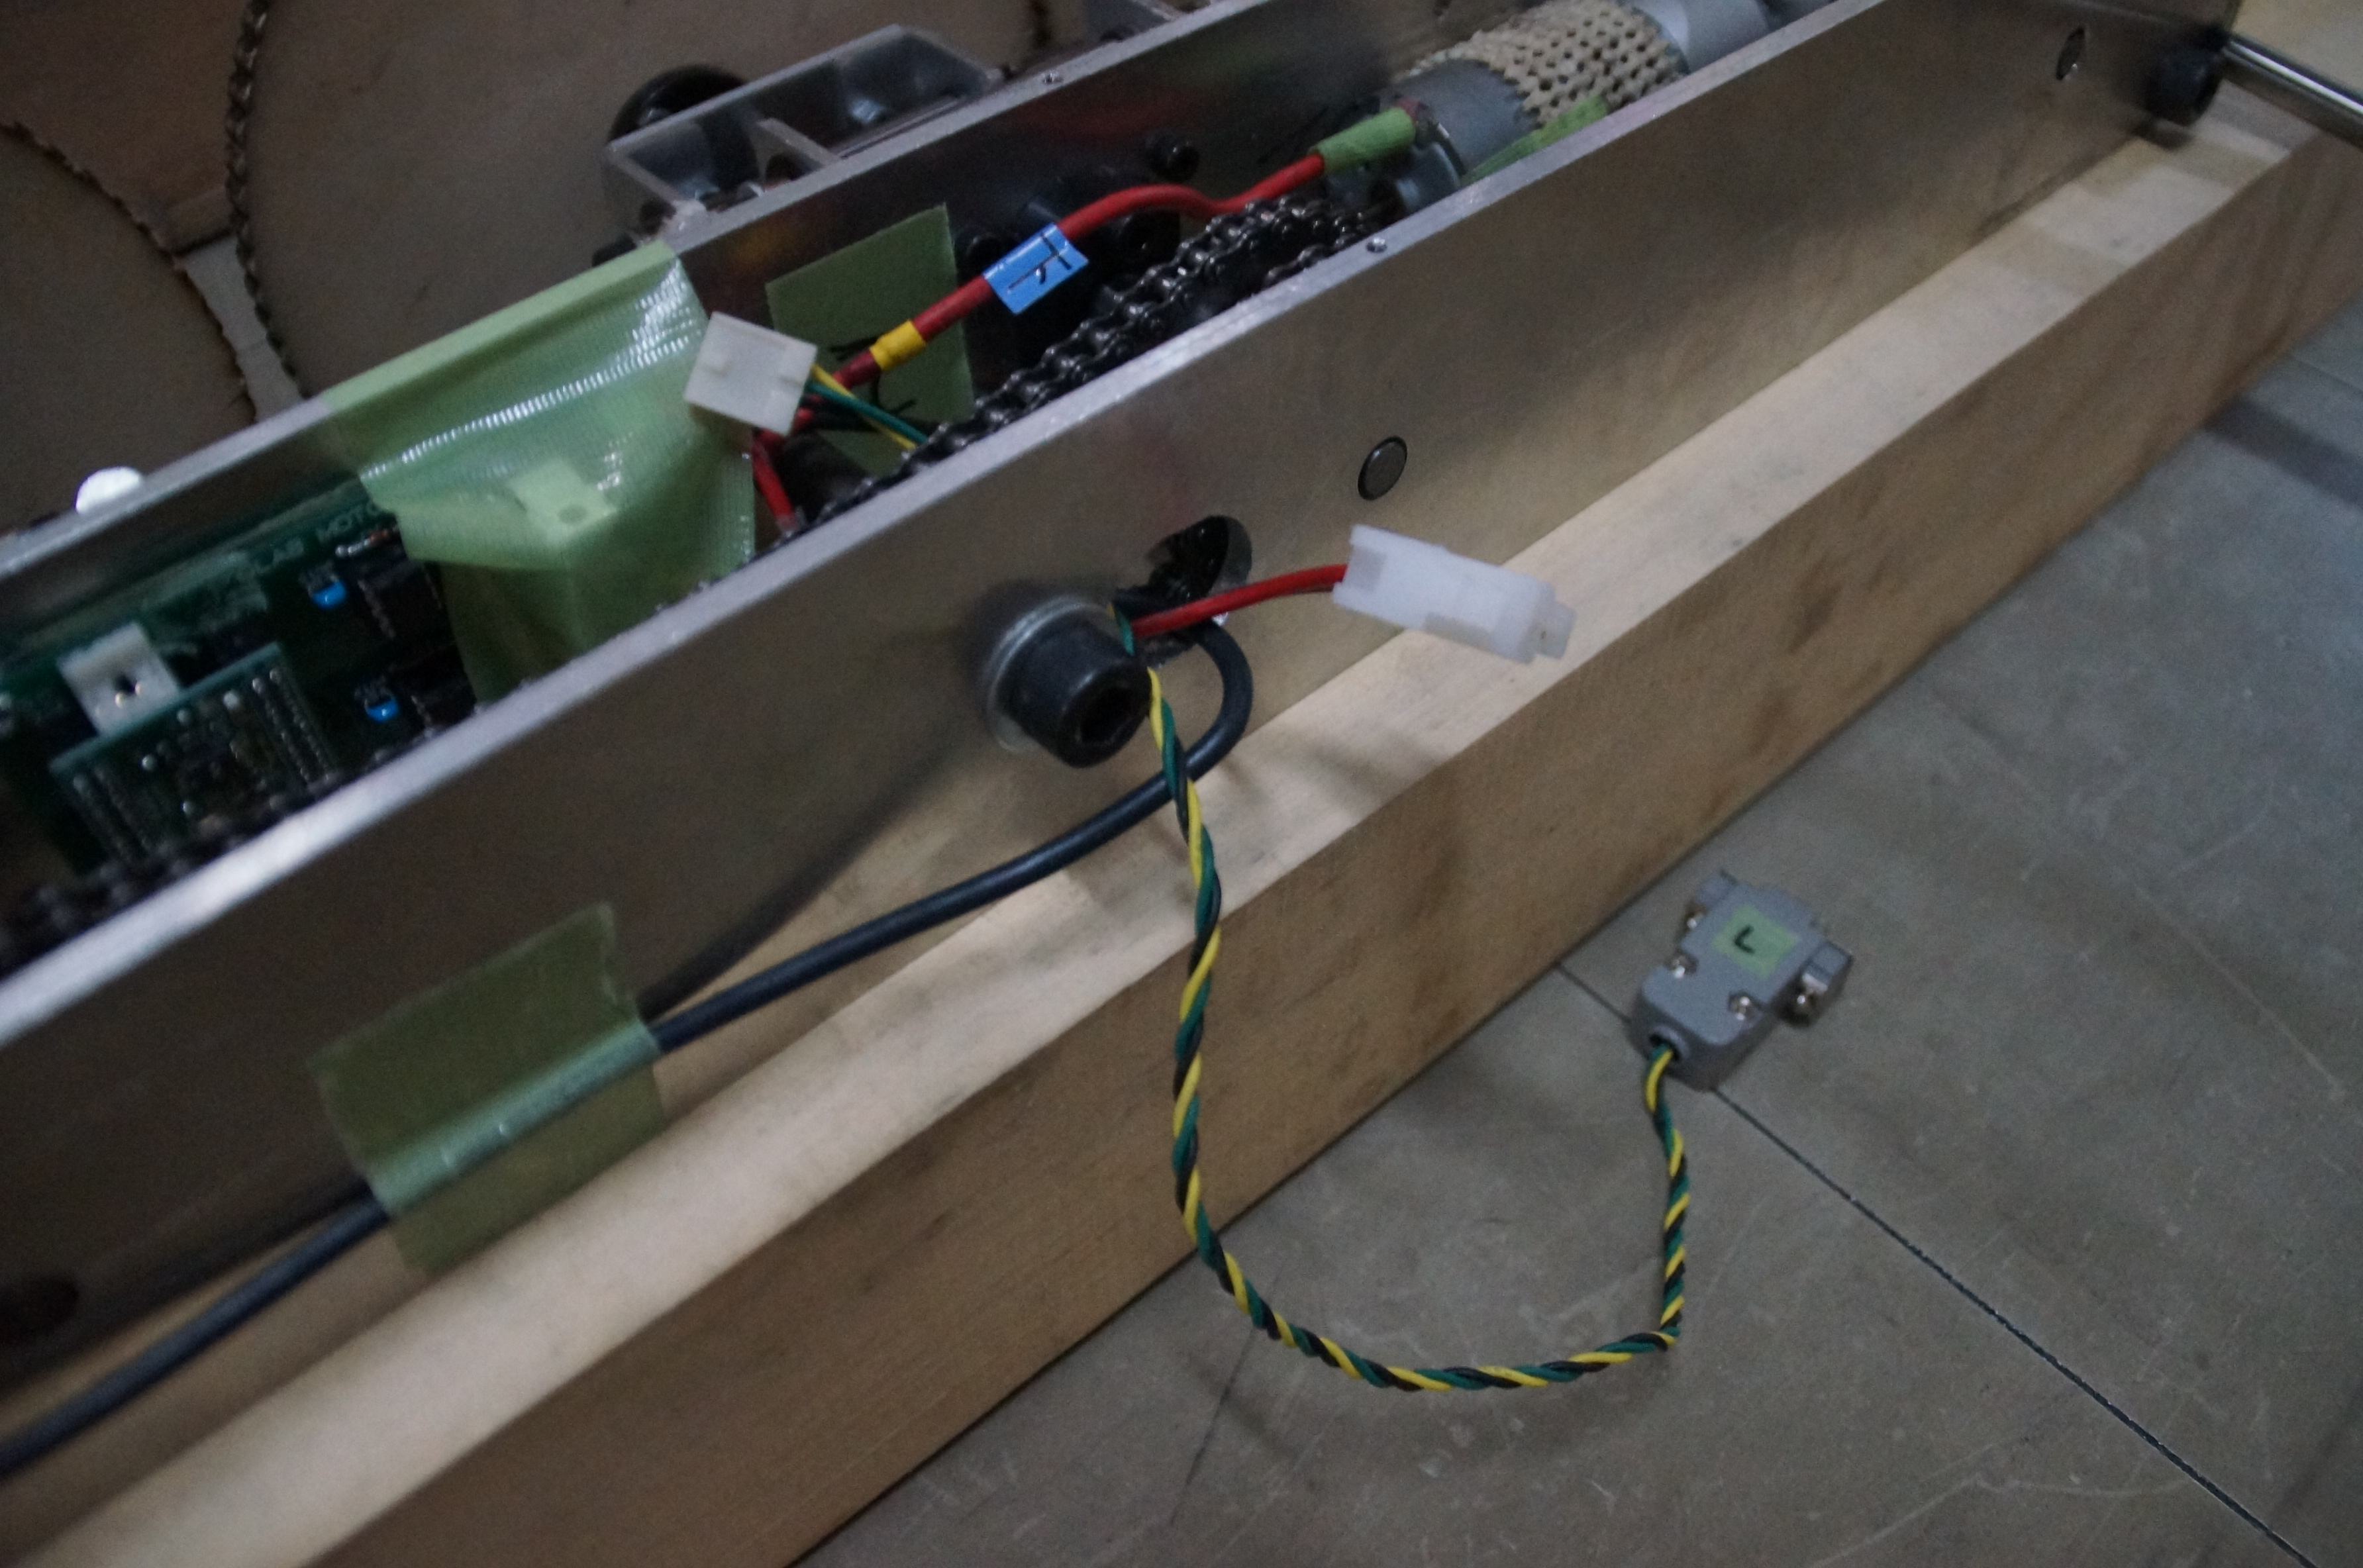
\includegraphics[width=80mm]{img/hard/f7.jpg}
  \caption{注意すべき配線}
  \label{fig:robot}%ここに文章中で使用する名前を指定する
 \end{center}
\end{figure}




\subsection{ポール分解}
ポールは支持パーツと操作パネル(カメラ内蔵)も接続されているため,それも分解する.ポールはM6のボルトを使用している.
\begin{enumerate}
 \item 底面に取り付けられている木の板を取り外し,支持パーツをスライドさせながら取り出す
 \item 操作パネルを保持するパーツを取り外し,操作パネルとポールを分離する 
 \item 操作パネルからカメラを取り外す
\end{enumerate}
支持パーツの中に1本だけ長いものがあるため,気をつけて整理する.
\begin{figure}[htp]
 \begin{center}
  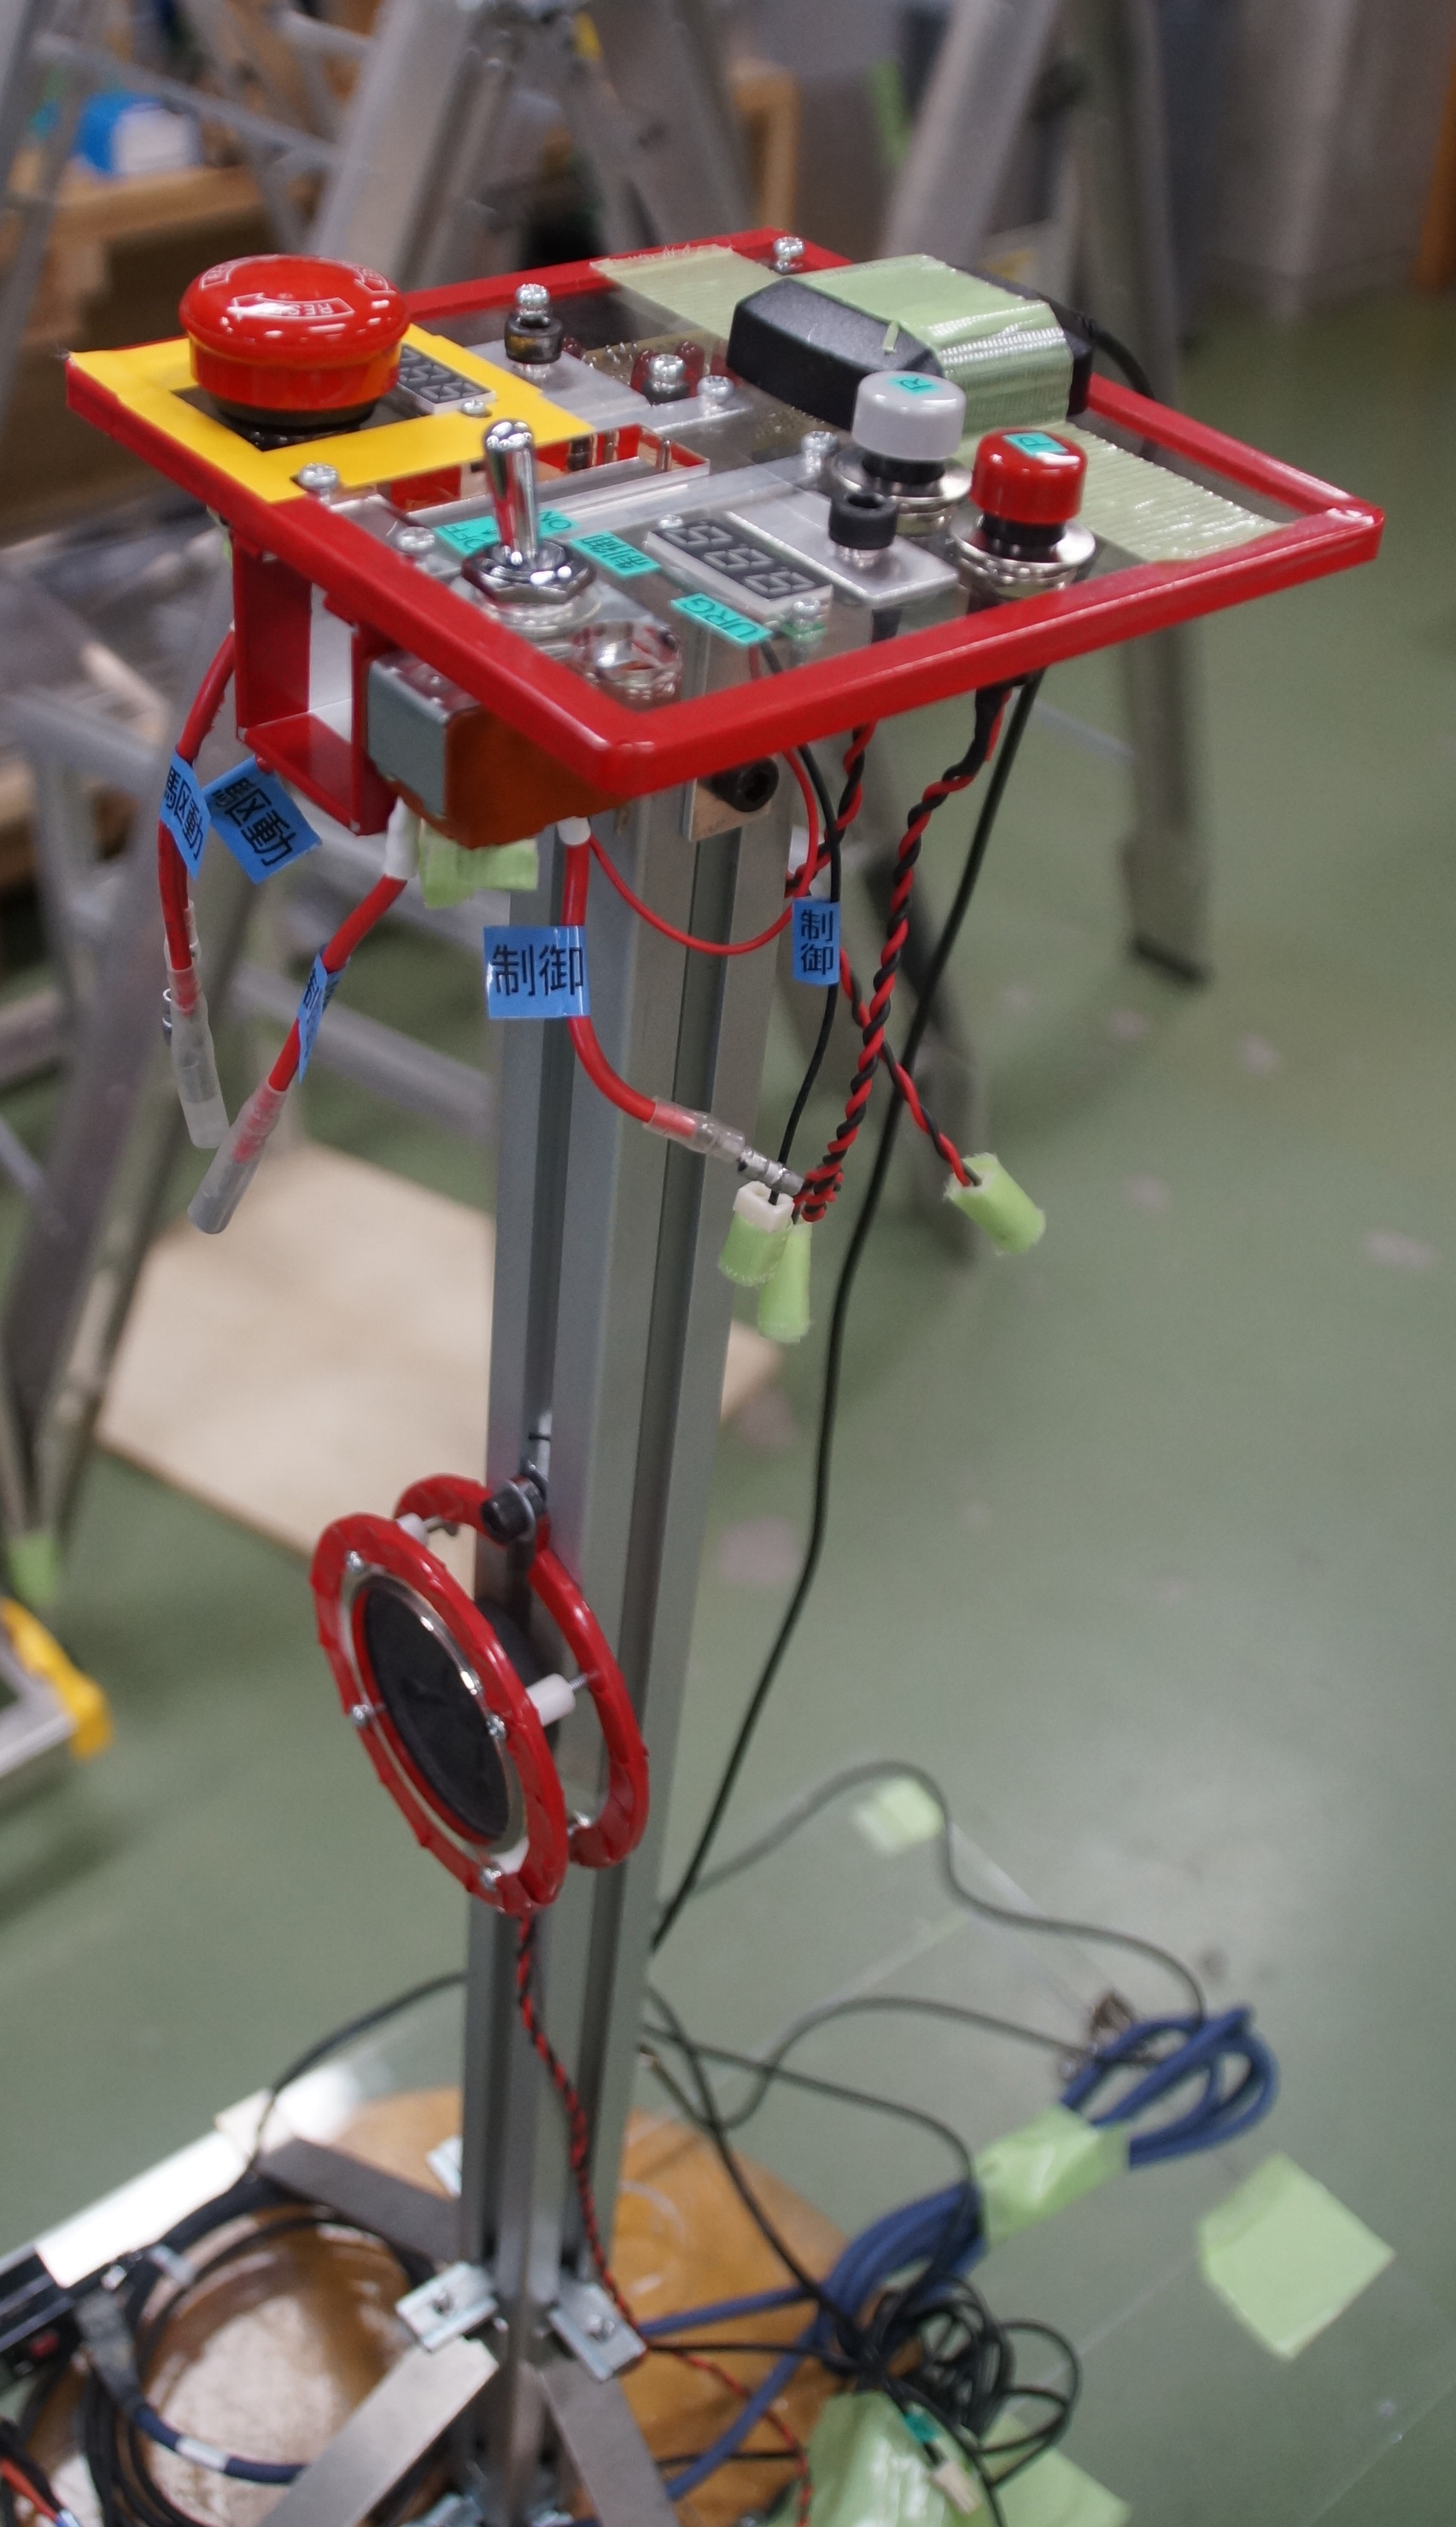
\includegraphics[width=80mm]{img/hard/f6.jpg}
  \caption{分解前}
  \label{fig:robot}%ここに文章中で使用する名前を指定する
 \end{center}
\end{figure}


\begin{figure}[htp]
 \begin{center}
  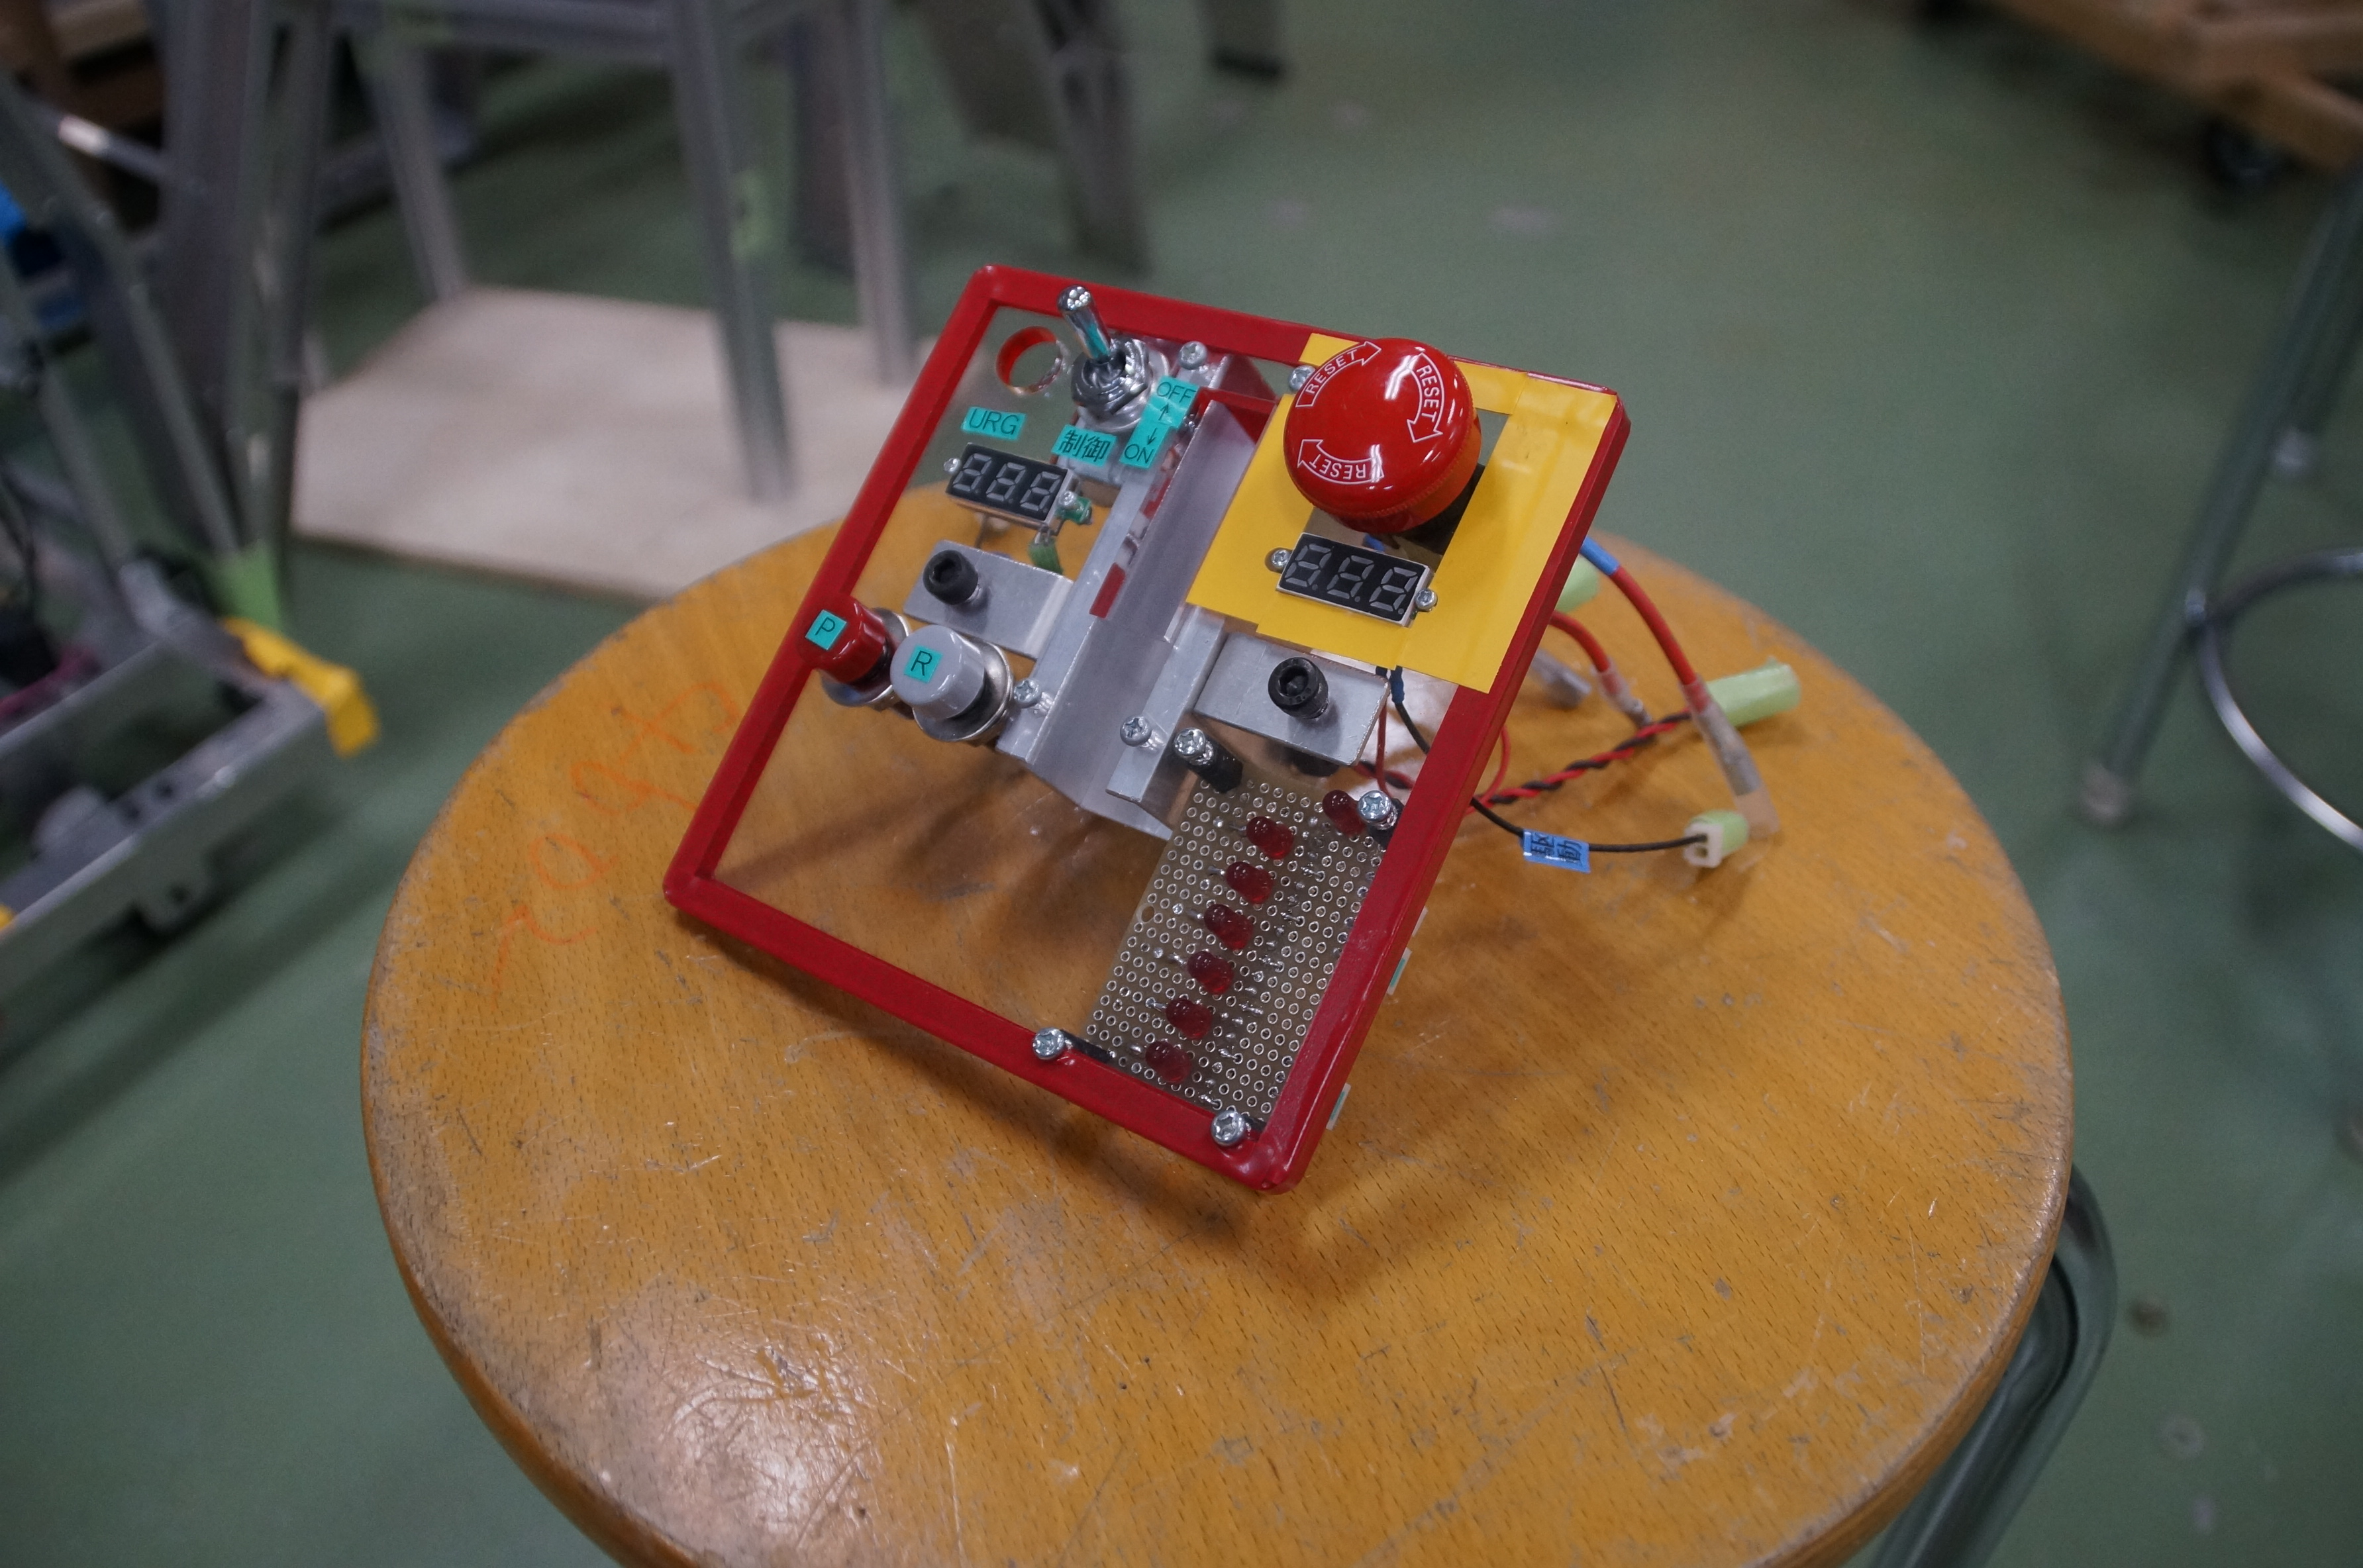
\includegraphics[width=80mm]{img/hard/f5.jpg}
  \caption{分解図}
  \label{fig:robot}%ここに文章中で使用する名前を指定する
 \end{center}
\end{figure}
\subsection{センサの取り外し}
上面アクリル板はモーションセンサと測域センサを取り付けてあるため,これも外し個包装を施す.

\subsection{箱つめ}
分解したD,Cモジュールを箱に詰める.詰める際にはCモジュールに接続されたセンサ関連は全て取り外し保管する.

